\subsection{Glyph: \glyph{And}}
\label{sec:and}


The output of an \glyph{and} glyph is True if all its inputs are True, and False otherwise.



\begin{glyphDescription}

\glyphSboTerm
SBO:0000173 ! and


\glyphIncoming One or more \glyph{logic arcs} (\sect{logicArc}).



\glyphOutgoing
One \glyph{logic arc} (\sect{logicArc}) or \glyph{modulation arc} (\sect{modulations}).


\glyphContainer
An \glyph{and} operator is represented by a circular shape containing the word ``AND''.
The shape is linked to two ports, that are small arcs attached to the centres of opposite sides of the shape, as shown in \fig{and}.
The incoming \glyph{logic arcs} (\sect{logicArc}) are linked to the extremity of the leftmost or uppermost port, while the outgoing \glyph{logic arc} (\sect{logicArc}) or \glyph{modulation} (\sect{modulation}) is linked to the extremity of the rightmost or bottommost port.

\glyphLabel
None.

\glyphAux
None.

\end{glyphDescription}

\begin{figure}[H]
  \centering
  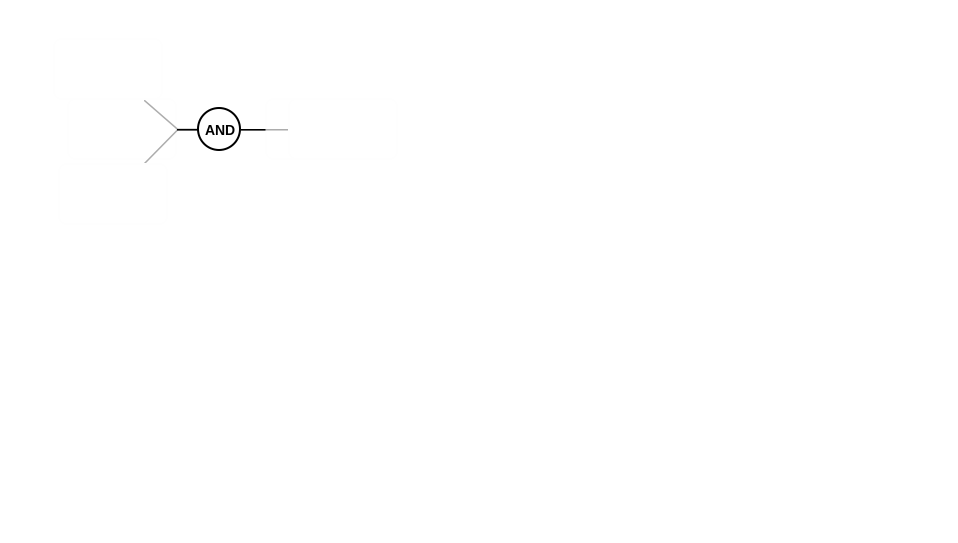
\includegraphics{images/and}
  \caption{The \PD glyph for \glyph{and}. Only two inputs are represented, but more would be allowed.}
  \label{fig:and}
\end{figure}

% The following maps illustrate the dephosphorylation of the MAP inase ERK by the protein phosphatase 2A and the STriatal Enriched Phosphatase, in ST (left) and ER (right).
%
% \begin{center}
% \scalebox{0.5}{\includegraphics{images/stimulation-example1}}
% \end{center}
